\begin{center}
Problema B

Brilho Cósmico

{\tiny Por Athos José}

Timelimit: $1$	
\end{center}

Na exploração fascinante do vasto universo, a medida das distâncias entre os corpos celestes e a apreciação de sua luminosidade, expressa através da magnitude, desempenham papéis cruciais. A distância é frequentemente quantificada em anos-luz, representando o tempo que a luz levaria para viajar da Terra à estrela em questão. A magnitude, por outro lado, é expressa em uma escala logarítmica que denota a luminosidade aparente de uma estrela. Nesta escala, quanto menor é o valor, mais luminosa é a estrela.

A ordenação das estrelas é uma tarefa crucial para os astrônomos e entusiastas do espaço, onde muitas das vezes é dada pela a magnitude aparente de uma estrela. Na Figura 1, podemos visualizar a estrela "Antares", conhecida como a principal estrela da constelação de Escorpião. Antares possui uma magnitude aparente de 0.91, sendo a estrela com a menor magnitude da constelação. Tal característica se reflete em sua notável visibilidade entre outras estrelas.

\begin{figure}[h!]
\centering
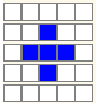
\includegraphics[width=4cm]{fig/e_1.png}
\label{B:1}
\caption{Constelação de Escorpião. Autor: Athos}
\end{figure}

Na mesma figura temos as estrelas ``EpsilonScorpii'' e ``DeltaScorpii'' que possuem uma magnitude aparente de 2,29. Para esses caso é comum utilizar a distância, onde, elas respectivamente possuem 65ly  e 402ly (sendo ly light-year ou ano-luz).

Nesta emocionante jornada cósmica, você é desafiado a criar um programa que organize as estrelas. Cada estrela é representada por um nome, uma distância em anos-luz e uma magnitude.

A tarefa é ordenar as estrelas em ordem crescente de magnitude aparente, levando em conta tanto os valores positivos quanto negativos. Em caso de empate nas magnitudes, as estrelas devem ser ordenadas em ordem decrescente pela a distância em relação à terra.

\vspace{0.3cm}
\textbf{Entrada}

A entrada consiste de um número inteiro $N$ $(1 \leq N \leq 10^5)$, representando o número de estrelas. Em seguida, seguem $N$ linhas, cada uma contendo a descrição de uma estrela no formato ``Nome Distancia Magnitude'', onde ``Nome'' é o nome da estrela (uma string sem espaços e com no máximo 50 caracteres), ``Distancia'' que é uma número inteiro representando a distância da estrela em anos-luz $(1 \leq Distancia \leq 10^9)$ e ``Magnitude'' é um número decimal representando a magnitude da estrela $(-40.0 \leq Magnitude \leq 40.0)$.

\vspace{0.3cm}
\textbf{Saída}

Seu programa deve imprimir os nomes da lista de estrelas ordenadas de acordo com as regras estabelecidas.

\begin{table}[h]
    \centering
    \begin{tabular}{|p{7cm}|p{7cm}|}
        \hline
        \begin{center}
            \vspace{-0.3cm}
            \textbf{Exemplos de Entrada}
            \vspace{-0.3cm}
        \end{center} 
         &  
        \begin{center}
            \vspace{-0.3cm}
            \textbf{Exemplos de Saída}
            \vspace{-0.3cm}
        \end{center} \\ \hline
         \texttt{6} & \texttt{Antares} \\  
         \texttt{KappaScorpii 464 2.39} & \texttt{LambdaScorpii} \\
         \texttt{EpsilonScorpii 65 2.29} &  \texttt{ThetaScorpii} \\
         \texttt{LambdaScorpii 703 1.62} &  \texttt{DeltaScorpii} \\
         \texttt{ThetaScorpii 272 1.86} &  \texttt{EpsilonScorpii} \\
         \texttt{Antares 553 0.91} &  \texttt{KappaScorpii} \\
         \texttt{DeltaScorpii 401 2.29} &  \\
         \hline
    \end{tabular}
    \caption{Exemplos de entradas e saídas}
    \label{tab:inputB}
\end{table}

\newpage

\begin{center}
\noindent
\lstinputlisting{abobora_23/B/B3.cpp}
\end{center}